\typeout{IJPHM template}
\typeout{Template version updated November 25, 2013}

% Please send questions regarding the Latex templates to Indranil Roychoudhury (indranil.roychoudhury@nasa.gov) or Matthew Daigle (matthew.j.daigle@nasa.gov).
 

\documentclass[IJPHM, 2014, 00]{PHMSociety}

%Declare Packages
\usepackage{graphicx}
\usepackage{amsmath}



\begin{document}

% Paper Title
\title{A Manuscript Template for the International Journal of Prognostics and Health Management}

% Authors List
\author{%			
	First Author\authorNumber{1}, Second Author\authorNumber{2}, and Third Author\authorNumber{3}
}

% Author Affiliations
\address{% This is a tabular environment so each affiliation needs to be separated by "\\" or "\tabularnewline"
	\affiliation{{1,2}}{First Business or Academic Affiliation 1, City, State, Zip Code, Country}{ %add emails
		{\email{author1@academic.edu}}\\ 
		{\email{author2@academic.edu}}
		} % emails input
	\tabularnewline % skip one row for next affiliation	
	\affiliation{3}{Second Business or Academic Affiliation 2, City, Province, Zip Code, Country}{ % add emails
		{\email{author3@academic.edu}}
		} % emails input
}



% Create the title
\maketitle
\pagestyle{fancy}
\thispagestyle{plain}


% PHM Society Distribution License Information, provide first author's name "FirstName LastName"
\phmLicenseFootnote{FirstAuthorFirstName FirstAuthorLastName}


% Abstract
\begin{abstract}%   %NOTE: Deleting the percentage after "{abstract}" may be lead to an extra leading space in the first line of the abstract, and this should be prevented.
Abstracts are required for all papers, and an abstract of 150-400 words should be included at the beginning of the paper. The abstract should be formatted as an unnumbered section and it is preferred to be presented in a single paragraph. Define all symbols and expand all abbreviations used in the abstract. Do not cite references in the abstract.
\end{abstract}



\section{Electronic Submission}
\label{sec:electr-subm} 
These instructions provide guidance for preparing papers for the publications of the Prognostics and Health Management Society. Use this document as a template if you are using \LaTeX. If Microsoft Word is preferred over \LaTeX, then download the corresponding Word Template from the conference webpage. The full text of the paper (except the title information, author information, and large figures and tables that need to span across two columns) is formatted in two-columns. Manuscripts should be written in clear, concise and grammatically correct English so that they are intelligible to a professional reader who is not a specialist in any particular field. Manuscripts that do not conform to these requirements and the following manuscript format will be returned to the author prior to review for correction. 
Use this template to prepare a two-column mock-up of your paper to show how your manuscript will appear in the proceedings of the conference. Where appropriate, use International System of Units (SI) only.


\section{General Guidelines}
The following section outlines general (non-formatting) guidelines to follow. These guidelines are applicable to all authors and include information on the policies and practices relevant to the publication of your manuscript.

\subsection{Publication by the Prognostics and Health Management Society}
Your manuscript cannot be published by the Prognostics and Health Management Society if:

\begin{enumerate}
	\item The work is classified or has not been cleared for public release. Authors are responsible for ensuring that papers are unclassified for public release and do not include sensitive or International Traffic in Arms Regulations (ITAR) export controlled (United States only) material.
	\item The work infringes copyright.
	\item The work has been published or is currently under consideration for publication elsewhere.
\end{enumerate}





\subsection{Copyright}
The Prognostic and Health Management Society advocates open-access to scientific data and uses a Creative Commons license (www.creativecommons.org) for publishing and distributing all papers. A Creative Commons license does not relinquish the authors' copyright; rather it allows them to share some of their rights with any member of the public under certain conditions whilst enjoying full legal protection. By submitting an article to Prognostics and Health Management Society publications, the authors agree to be bound by the associated terms and conditions including the following:
As the author, you retain the copyright to your work. By submitting your Work, you are granting anybody the right to copy, distribute and transmit your Work and to adapt your Work with proper attribution under the terms of the Creative Commons Attribution 3.0 United States license. You are also granting worldwide, non-exclusive, and irrevocable rights to the Prognostics and Health Management Society to publish and disseminate your work through electronic and print media if it is accepted for publication. A license note citing the Creative Commons Attribution 3.0 United States License needs to be placed in the footnote on the first page of the article.




\section{Paper Format}
Papers size should be ``US Letter'' (8.5 by 11 inches; 215.9 mm x 279.4 mm), with two-column format, except for the title, author information and figures and tables placed after the references. Margins should be 1.0 inches top and bottom, and 0.75 left and right. An exception is for the first page who top margin needs to be 1.5 inches. Columns should be equally sized, 3.38 inches, with 0.25 inches between columns. Paragraphs should be unindented, with a 6-point vertical spacing between paragraphs. All papers should use Times Roman 10-point font throughout.



\subsection{Title and Author Information}
All items in the title block should be centered across both columns.  The title should be set in 17 pt bold, with a 14 pt space below.  The author's names should be set in 11 pt font, with an 11 pt space below. The paper title should be in the ``Title Case'' or ``Headline Style'', i.e., capitalized the first and last words of the title and all nouns, pronouns, adjectives, verbs, adverbs, and subordinating conjunctions (such as, `if', `because', `as', `that', and so on). For example, the title of the paper should be ``A Manuscript Template for the European Conference of the Prognostics and Health Management Society 2014" instead of ``A manuscript template for the European conference of the prognostics and health management society 2014'' or ``A Manuscript Template For The European Conference Of The Prognostics and Health Management Society 2014''.

For each author, a numbered superscript should be used to indicate institutional affiliation. Following the author information, each institution with which any of the authors are affiliated should be listed, including addresses. These should be indicated by superscripts as well, and set in 9 pt italic, with a 12 pt space below the final one. The final item in the title block is the author's email address in 9 pt italics.  A 24 pt space should follow this line.


\subsection{Section and Subsection Headings}

Section and subsection headings are numbered using Arabic numerals separated by a period (`.'). Section headings (\verb+\section+, in \LaTeX) are ``small capitals'', 10 pt, boldface, and flush left. Subsections (\verb+\subsection+, in \LaTeX) are 10 pt, boldface, and flush left.  Sub-subsections (\verb+\subsubsection+, in \LaTeX) are 10 pt, boldface, and flush left.  All levels below this are unnumbered, 10pt, boldface, with text beginning immediately following the heading on the same line. Insert a new line after each section.

\subsection{Tables and Figures}
Tables and figures should be center aligned. %If possible, place figures and tables at the top and bottom of columns, and avoid placing them in the middle of columns. Large figures and tables may span across columns. 
Table captions should appear above the tables. Insert figures and tables after they are cited in the text. Table captions should be 10 pt, in sentence case, and centered with respect to the table. Two-column-wide figures and tables may be used as appropriate. Tables should be self-contained and complement, but not duplicate, information contained in the text. See the Table~\ref{table1} example for table style and column alignment. 


\begin{table}[t] \small  
	\begin{center}  
		
	\caption{Title of the table.}
		\label{table1}
	
	\begin{tabular}{ l | l }
		\hline \hline
		\textbf{Time}	& \textbf{Event}              \\ 
		\hline \hline
		15:56:21.194	& Start of scenario  \\ \hline
		15:56:21.236	& Sample of sensors  \\ \hline
		15:56:21.736	& Sample of sensors  \\ \hline
		...           &                    \\ \hline
		15:56:21.736	& Sample of sensors  \\ \hline
		15:56:21.736	& Fault injection  \\ \hline
		15:56:21.736	& Sample of sensors  \\ \hline
		...           &                    \\ \hline
		15:57:22.252	& End of scenario    \\ \hline
	\end{tabular}
	\end{center}
\end{table}


Place figure captions below all figures. If your figure has multiple parts, include the labels ``a),'' ``b),'' etc., below and to the left of each part, above the figure caption. Please verify that the figures and tables you mention in the text actually exist. Number each different type of illustration (i.e., figures, tables, images) sequentially with relation to other illustrations of the same type.

The size of the font in the figure must match the size of the font in the manuscript text; it must be legible and not blurred or pixelated. The line weight of figures must not appear broken or rasterized. For vector graphics, the preferred format is EPS; for halftones, please use TIFF format. Vector graphics containing fonts must have the fonts embedded in the files. Do not use faint lines and/or lettering and check that all lines and lettering within the figures are legible at final size. All lines should be at least 0.1 mm (0.3 pt) wide. Scanned line drawings and line drawings in bitmap format should have a minimum resolution of 300 dpi. Color figures are acceptable but you must ensure that data are distinguishable in grayscale prints.

\subsubsection{Figure Styles}
When creating figures, there are several formatting guidelines which should be followed:
\begin{itemize}
\item do not put a frame around the figure outside the axes
\item do not color the background of a figure
\item	do not use pie charts
\item	do not used ``stacked bar'' charts
\item	do not use any sort of ``3d'' effect in figures
\item	do always include a clear and distinct legend
\item	avoid using only color to distinguish data (i.e., use point and line shapes)
\item	where possible, make figures entirely in grayscale
\end{itemize}

Note that the default settings for Microsoft Excel violate many of these guidelines, and more generally, it is quite difficult to create publication-quality figures using Excel.

\begin{figure}[t]
\centering
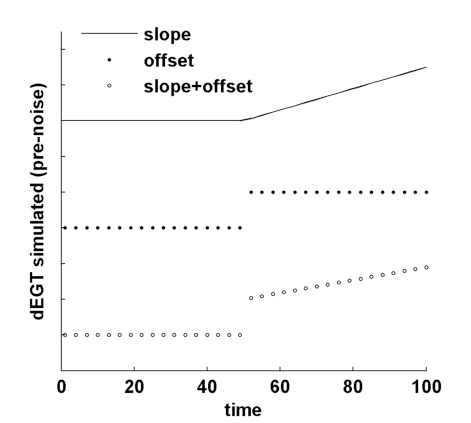
\includegraphics[scale=.9]{figure1}
\caption{This is an example of a figure caption.}
\label{fig:pastedGraphic}
\end{figure}



\subsection{Equations, Numbers, Symbols, and  Abbreviations}

Equations are centered and numbered consecutively, with equation numbers in parentheses flush right, as in Eq.~(\ref{eq:one}). Insert a blank line on either side of the equation. First use the equation editor to create the equation.
A sample equation is included here, formatted using the preceding instructions. To make your equation more compact, you can use the solidus (/) or appropriate exponents when the expression is five or fewer characters.  Use parentheses to avoid ambiguities in denominators.


\begin{equation}
\int^{a}_{b}F(x)\,dx = 2\sigma
\label{eq:one}
\end{equation}


Be sure that the symbols in your equation are defined before the equation appears, or immediately following. Italicize symbols (T might refer to temperature, but T is the unit tesla). In the text, refer equations as ``Eq.~(\ref{eq:one})'' and not as ``(\ref{eq:one})'' or ``equation~(\ref{eq:one})'', except at the beginning of a sentence where ``Equation~(\ref{eq:one})'' can be used. Equations can be labeled other than ``Eq.'' should they represent inequalities, matrices, or boundary conditions. If what is represented is really more than one equation, the abbreviation ``Eqs.'' can be used.

Define abbreviations and acronyms the first time they are used in the main text. Very common abbreviations such as PHM and SI do not have to be defined. Abbreviations that incorporate periods should not have spaces: write ``P.R.'', not ``P. R.'' Delete periods between initials if the abbreviation has three or more initials; e.g., U.N. but ESA. Do not use abbreviations in the title unless they are unavoidable.

\subsection{Citing Literature}

\subsubsection{References in Text}
The following entries are intended to provide examples of the different reference types, in accordance with the Annual Conference of Prognostic and Health Management Society style. All references should be in 10-point font.

Works by a single author are cited by the last name of the author and the year of publication are inserted in the text at the appropriate point, e.g., ``early work on this topic~\cite{ferrell}''. If the name of the author or the date appear as part of the narrative, cite only missing information in parentheses, e.g., ``in her early work,~\cite{ferrell} found''.

When a work has two authors, always cite both names every time the reference occurs in the text. In parenthetical material join the names with an ampersand (\&), e.g., ``as has been shown~\cite{Schwabacher}''. However, in narrative text, join the names with the word ``and'', e.g., ``\cite{Schwabacher} show that''. 

When a work has three, four, or five authors, cite all authors the first time the reference occurs, e.g., ``\cite{vachtsevanos} found''. In all subsequent citations, include only the surname of the first author followed by ``et al.'' (Latin for ``and others'') and the year of publication, e.g., ``\shortcite{vachtsevanos} found''. 

Works by associations, corporations, government agencies, etc. are referenced by the name of the body that created the work, e.g., ``the 2004 International Organization for Standardization [ISO] report''. When appropriate, abbreviations can be used in all subsequent citations, provided that there is enough information in the text citation for a reader to locate its source in the reference list without difficulty, e.g., ``the report ~\cite{iso} showed''.





\subsubsection{Formatting the ``References'' Section}

Note that if you use a ``.bib'' file for bibliography, you have to first run the following command to generate the corresponding``.bbl'' file. Hence, if your bibliography file is called ``phm.bib'', the first execute the following:

\textit{bibtex phm} 

This would generate the file ``phm.bbl''. Then you can compile the rest of your ``.tex'' file(s) to get the pdf output. If you have multiple bibliography files, follow the above to generate the corrsponding ``.bbl'' files for all of them. 

For proper reference style use the following guidelines to create your ``.bib'' file:

\begin{enumerate}
\item Articles in periodicals should be referred using @ARTICLE or @Article \cite{wunsch}. For periodicals all of the preceding information is required. The journal issue number is preferred, but the month (Nov.) can be substituted if the issue number is not available. Use the complete date for daily and weekly publications. Transactions follow the same style as other journals; if punctuation is necessary, use a colon to separate the transactions title from the journal title.
\item For books used @BOOK or @Book to get the format showed in~\cite{bhattacharyya}. An example has been provided in ``phm.bib'' file included in this latex package.
\item Articles in conference proceedings should be referred using @INPROCEEDINGS or @InProceedings \cite{ferrell}.
\item Dissertations should be referred using @PHDTHESIS or @PhDThesis \cite{chen}.
\end{enumerate}


Electronic publications, CD-ROM publications and regularly issued, dated electronic journals are permitted as references. Archived data sets also may be referenced as long as the material is openly accessible and the repository is committed to archiving the data indefinitely. References to electronic data available only from personal Web sites or commercial, academic, or government ones where there is no commitment to archiving the data are not permitted in the reference list. Some references have a Digital Object Identifier (DOI) - a string of numbers (and/or letters) assigned to individual journal articles as well as to some other publications. Include the DOI for articles that you retrieve both online and in hardcopy. The database may provide the DOI as part of the citation, or you may have to look at the top or bottom of the first page of the article to find it.


%\vspace{1in}


\section{Conclusion}
Although a conclusion may review the main points of the paper, it must not replicate the abstract. A conclusion might elaborate on the importance of the work or suggest applications and extensions. Note that the conclusion section is the last section of the paper to be numbered. The appendix (if present), acknowledgment, and references are listed without numbers.



\section*{Acknowledgment}
The acknowledgment section is optional and if present, should be unnumbered. Please list any acknowledgment here using a single paragraph.




\section*{Nomenclature}
Note that this section is optional.

\begin{tabular}{ l  l }
	$A$			&amplitude of oscillation\\ 
	$a$			&acceleration\\ 
	$Cp$		&pressure coefficient\\ 
	$Fx$			&X component of the resulting force\\  
	$Fy$			&Y component of the resulting force\\ 
	$m$			&mass\\ 
	$dt$			&time step\\ 
	$T$  	   		&temperature \\ 
	$P$	   		&pressure \\ 
	$f, g$      		&generic functions\\ 
	$h$	   		&height\\ 
	    $I$   	   	&current\\ 
	$V$	   		&voltage\\ 
	$\alpha$      	&dummy variable\\ 
 \end{tabular}





% Bibliography
% ---------------------------------------------------------------------------------
\bibliographystyle{apacite}
\PHMbibliography{ijphm}
% ---------------------------------------------------------------------------------


\section*{Biographies}

\begin{wrapfigure}[8]{l}[0pt]{0.7in}
\vspace{-15pt}
\begin{center}
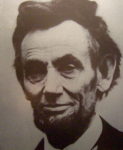
\includegraphics[width=0.83in,height=1in,clip,keepaspectratio]{abe}
\end{center}
\end{wrapfigure}
\noindent\textbf{First A. Author} and the other authors may include biographies at the end of regular papers. The biography paragraph may contain a place and/or date of birth (list place, then date). Next, the author's educational background is listed. The degrees should be listed with type of degree in what field, which institution, city, state, and country, and year degree was earned. Please use the pronoun of the person (he or she) and not the author's last name. Military and work experience, including summer and fellowship jobs may also be listed. Information concerning previous publications may be included. Current and previous research interests end the paragraph. Finally, list any memberships in professional societies other than the PHM Society followed by any awards and honors. If a photograph is provided, the biography will be indented around it. The photograph is placed at the top left of the biography.


\noindent\textbf{Second B. Author} This format should be used if no pictures are used for the biographies. Other authors may include biographies at the end of regular papers. The biography paragraph may contain a place and/or date of birth (list place, then date). Next, the author's educational background is listed. The degrees should be listed with type of degree in what field, which institution, city, state, and country, and year degree was earned. Please use the pronoun of the person (he or she) and not the author's last name. Military and work experience, including summer and fellowship jobs may also be listed. Information concerning previous publications may be included. Current and previous research interests end the paragraph. Finally, list any memberships in professional societies other than the PHM Society followed by any awards and honors.

\section*{Appendix}

If the paper has an appendix, the appendix should appear at the end of the paper after the biographies. The appendix section is optional. 

\end{document}


